\documentclass[fleqn,10pt]{wlscirep}
\usepackage[utf8]{inputenc}
\usepackage[T1]{fontenc}
\usepackage{lineno}
\usepackage{adjustbox}
\usepackage{multirow}
% \usepackage{hyperref}
% \usepackage{academicons}
% \usepackage{xcolor}

% \newcommand{\orcid}[1]{\href{https://orcid.org/#1}{\textcolor[HTML]{A6CE39}{\aiOrcid}}}

\linenumbers

\title{A longitudinal dataset of childhood gut microbiome linked with cognitive evaluation}

\author[1]{Kevin S Bonham}
\author[1]{Shelley Hoeft McCann}
\author[1]{Sophie Rowland}
\author[2]{Alexandra R. Volpe}
\author[2]{Kellyn Dyer}
\author{RESONANCE Consortium}
\author[2,3]{Viren D’Sa}
\author[2,3,5,6]{Sean C. L. Deoni}
\author[1,*]{Vanja Klepac-Ceraj}

\affil[1]{Department of Biological Sciences, Wellesley College, Wellesley, MA, 02481, USA}
\affil[2]{Advanced Baby Imaging Lab, Hasbro Children’s Hospital, Rhode Island Hospital, Providence, RI, 02903, USA}
\affil[3]{Department of Pediatrics, Warren Alpert Medical School at Brown University, Providence, RI, 02912, USA}
\affil[5]{Department of Radiology, Warren Alpert Medical School at Brown University, Providence, RI, 02912, USA}
\affil[6]{Maternal, Newborn, and Child Health Discovery \& Tools, Bill \& Melinda Gates Foundation; Seattle WA, USA}

\affil[*]{corresponding author: Vanja Klepac-Ceraj (vklepacc@wellesley.edu)}


\begin{abstract}
Early childhood is shaped by numerous genetic and environmental factors.
Exposures in early life can have profound effects on neural, cognitive, and immunological development, but identifying relationships between exposure and outcome, especially when many factors have small effects, can be challenging.
Here we provide a partially longitudinal dataset of early childhood gut microbiomes from XXX unique children from birth through adolescence, combined with rich demographic data and cognitive assessments.
Microbiomes were sequenced using both shotgun metagenomic sequencing as well as 16S rRNA amplicon sequencing, enabling more direct comparisons with existing child microbiome data as well as within-cohort assessment of relationships between the microbiome, demographic background, and cognitive development

\end{abstract}
\begin{document}

\flushbottom
\maketitle
\thispagestyle{empty}

\noindent Please note: Abbreviations should be introduced at the first mention in the main text – no abbreviations lists or tables should be included.
Structure of the main text is provided below


\section*{Background \& Summary}

The first years of life are a unique and dynamic period of neurological and cognitive development.
Throughout childhood, a child’s brain undergoes remarkable anatomical, microstructural, organizational, and functional change.
By age 5, a child’s brain has reached over 85\% of its adult size,
has achieved near-adult levels of myelination,
and the pattern of axonal connections has been established \cite{Silbereis2016-lp}
This development is profoundly affected by the child’s environment and early life exposures \cite{Fox2010-lp}.
The first years of life also witness dramatic changes in the gut microbiome.
The gut microbial community is seeded at birth
and develops over the course of the first year from a low-diversity community
dominated by Firmicutes and Proteobacteria,
to a more diverse, adult-like microbiome upon the introduction of solid food.
This microbial community development is also shaped by the environment,
with factors such as mode of delivery and diet
(breast milk vs formula) known to have lasting effects on community composition \cite{Backhed2015-ko, Dominguez-Bello2010-ti}

The gut, the gut microbiome, and the central nervous system are intricately linked
through a system known as the gut-microbiome-brain axis \cite{Clarke2013-yu},
and differences in microbial communities are associated with, and in some cases cause,
changes in neurocognitive development \cite{Flannery2020-de, Gao2019-je}
and the outcome of neurological disorders such as autism \cite{Sharon2019-ak}.
However, the study of the relationships between environmental exposures, neurocognitive development,
and the gut microbiome during neurotypical development remains in its infancy \cite{Carlson2018-iw,Sordillo2019-wi}

Here, we collected data on microbial taxonomic and functional composition
of the childhood microbiome paired with demographic information about participants
and age-appropriate cognitive assessments that produce IQ-like measures of motor, language, and social development.
Historically, many studies investigating the microbiome have used amplicon sequencing of conserved genes (eg 16S rRNA),
while more recently there has been a shift towards using shotgun metagenomic sequencing
which can provide more granular taxonomic assignment, including identification of fungal and viral components,
and direct evidence for gene functional potential..
Here, we provide both amplicon (16S rRNA V4-V5) and shotgun metagenomic sequencing
to enable the greatest potential for comparisons with previous studies
as well as the higher resolution enabled by sequencing the entire metagenome.
Understanding how the gut microbiome of healthy children
interacts with the complex metabolism of these and other neuroactive molecules
will be critical in understanding the etiology of neurocognitive disorders
and how to promote healthy neurological development.



\section*{Methods}

\subsection*{Human Subjects}

Data used in this study were drawn from the ongoing longitudinal RESONANCE study
of healthy and neurotypical brain and cognitive development,
based at Brown University in Providence, RI, USA.
RESONANCE is part of the NIH initiative Environmental influences on Child Health Outcomes (ECHO) \cite{Forrest2018-ud,Gillman2018-om},
a longitudinal observational study of healthy and neurotypical brain development
that spans the fetal and infant to adolescent life stages,
combining neuroimaging (magnetic resonance imaging, MRI), neurocognitive assessments, bio-specimen analyses, subject genetics,
environmental exposures such as lead, and rich demographic, socioeconomic, family and medical history information.
From the RESONANCE cohort, 344 typically-developing children
between the ages of 28 days and 15 years oldwere selected for analysis in this study. 

General participant demographics are provided in Tables \ref{tab:demographics} \ref{tab:agestats} and Figure \ref{fig:data}.
Complete metadata are available in Data Records (see below), with children being representative of the RI population.
As a broad background, children in the RESONANCE cohort were born full-term (>37 weeks gestation)
with height and weight normal for gestational age, and from uncomplicated singleton pregnancies.
Children with known major risk factors for developmental abnormalities at enrollment were excluded.
In addition to screening at the time of enrollment,
on-going screening for worrisome behaviors using validated tools was performed
to identify at-risk children and remove them from subsequent analysis.

Exclusion criteria included: in utero exposure to alcohol, cigarette or illicit substance exposure;
preterm (<37 wks gestation) birth; small for gestational age or less than 1500 g; fetal ultrasound abnormalities;
preeclampsia, high blood pressure, or gestational diabetes; 5 minute APGAR scores <8;
NICU admission; neurological disorder (e.g., head injury resulting in loss of consciousness, epilepsy);
and psychiatric or learning disorder (including maternal depression) in the infant, parents, or siblings requiring medication in the year prior to pregnancy.

Demographic and other non-biospecimen data such as race and ethnicity, parental education and occupation,
feeding behavior (breast- and formula-feeding), child weight and height,
were collected through questionnaires or direct examination as appropriate.
All data were collected at every assessment visit.
All procedures for this study were approved by the local institutional review board at Rhode Island Hospital,
and all experiments adhered to the regulation of the review board.
Written informed consent was obtained from all parents or legal guardians of enrolled participants.


\subsection*{Cognitive Assessments}

Overall cognitive function was assessed using age-appropriate methods.
For children from birth to 30 months, we used an Early Learning Composite
as assessed via the Mullen Scales of Early Learning (MSEL) \cite{Mullen1995-ty},
a standardized and population-normed tool for assessing fine and gross motor,
expressive and receptive language, and visual reception functioning in children from birth through 68 months of age.

The third edition of the Bayley Scales of Infant and Toddler Development \cite{Bayley2006-wm}
is a standard series of measures used primarily to assess the development of infants and toddlers,
ranging from 1 to 42 months of age.

The Wechsler Intelligence Quotient for Children (WISC) \cite{Wechsler2012-mi}
is an individually administered standard intelligence test for children aged 6 to 16 years.
It derives a full scale intelligence quotient (IQ) score, which we used to assess overall cognitive functioning.
The fourth edition of the Wechsler Preschool and Primary Scale of Intelligence (WPPSI-IV) \cite{Wechsler2012-mi}
is an individually administered standard intelligence test for children aged 2 years 6 months to 7 years 7 months,
trying to meet the increasing need for the assessment of preschoolers.
Just as the WISC, it derives a full scale IQ score, which we used to assess overall cognitive functioning.


\subsection*{Stool Sample Collection and Sequencing}

Stool samples (n=493) were collected by parents in OMR-200 tubes (OMNIgene GUT, DNA Genotek, Ottawa, Ontario, Canada),.
immediately stored on ice, and brought within 24 hrs to the lab in RI where they were immediately frozen at -80$^{\circ}$C.
Stool samples were not collected if the subject had taken antibiotics within the last two weeks.
DNA extraction was performed at Wellesley College (Wellesley, MA).
Nucleic acids were extracted from stool samples using the RNeasy PowerMicrobiome kit
automated on the QIAcube (Qiagen, Germantown, MD), excluding the DNA degradation steps.
Extracted DNA was sequenced at the Integrated Microbiome Resource (IMR, Dalhousie University, NS, Canada)

Shotgun metagenomic sequencing was performed on all samples.
A pooled library (max 96 samples per run) was prepared using the Illumina Nextera Flex Kit for MiSeq and NextSeq from 1 ng of each sample.
Samples were then pooled onto a plate and sequenced
on the Illumina NextSeq 550 platform using 150+150 bp paired-end “high output” chemistry,
generating ~400 million raw reads and ~120 Gb of sequence per plate.

For sequencing 16S rRNA gene amplicons,
the V4-V5 region of the 16S ribosomal RNA gene was sequenced according to the protocol
described by Comeau et al. \cite{Comeau2017-jg}.
Briefly, the V4-V5 region was amplified once using the Phusion High-Fidelity DNA polymerase
(ThermoFisher Scientific, Waltham, MA) and universal bacterial primers
515F: 5’-GTGYCAGCMGCCGCGGTAA-3’ and 926R: 5’-CCGYCAATTYMTTTRAGTTT-3’ \cite{Parada2016-uz,Walters2016-fi}.
These primers had appropriate Illumina adapters and error-correcting barcodes unique to each sample
to allow up to 380 samples to be simultaneously run per single flow cell.
After being pooled into a single library and quantified fluorometrically,
samples were cleaned-up and normalized using the high-throughput Charm Biotech Just-a-Plate 96-well Normalization Kit (Charm Biotech, Cape Girardeau, MO).
The normalized samples were sequenced on the Illumina MiSeq platform (Illumina, San Diego, CA)
using 300+300 bp paired-end V3 chemistry, producing ~55,000 raw reads per sample.

\subsection*{Computational Analysis}

Shotgun metagenomic sequences were analyzed using the bioBakery suite of computational tools (McIver et al. 2018).
First, \verb|KneadData| (v0.7.7) was used to perform quality control of raw sequence reads,
such as read trimming and removal of reads matching a human genome reference.
Next, \verb|MetaPhlAn| (v3.0.7, using database \verb|mpa_v30_CHOCOPhlAn_201901|) was used to generate taxonomic profiles
by aligning reads to a reference database of marker genes.
Finally, \verb|HUMAnN| (v3.0.0a4) was used to functionally profile the metagenomes.

Raw amplicon sequences were profiled using Quantitative Insights in Microbial Ecology 2 (QIIME2) v2021.2.0 (Bolyen et al. 2019).
Briefly, primers flanking V4-V5 were removed from fastq reads using the cutadapt (v3.2) QIIME2 plugin (Martin 2011).
Raw sequence reads of samples from enrichment cultures were denoised, filtered and clustered into amplicon sequence variants (ASVs) using the Divisive Amplicon Denoising Algorithm (DADA2) plugin in QIIME 2 (Callahan et al. 2016).
After denoising and filtering, 16270 total sequences were recovered with a mean length of 373 bases (270-465, standard deviation 13.21).
Taxonomy was assigned to each ASV using a Naïve-Bayes classifier compared against SILVA v.138 reference database (Yilmaz et al. 2013; Quast et al. 2013) trained on the 515F-806R region of the 16S rRNA gene (Bokulich et al. 2018)

Additional data processing, generation of summary statistics, and generation of plots was performed using the julia programming language.
See Code Availability section for additional details.

\section*{Data Records}

% The Data Records section should be used to explain each data record associated with this work, including the repository where this information is stored, and to provide an overview of the data files and their formats 
% Each external data record should be cited numerically in the text of this section, for example \cite{Hao:gidmaps:2014}, and included in the main reference list as described below 
% A data citation should also be placed in the subsection of the Methods containing the data-collection or analytical procedure(s) used to derive the corresponding record 
% Providing a direct link to the dataset may also be helpful to readers (\hyperlink{https://doi.org/10.6084/m9.figshare.853801}{https://doi.org/10.6084/m9.figshare.853801})


% Tables should be used to support the data records, and should clearly indicate the samples and subjects (study inputs), their provenance, and the experimental manipulations performed on each (please see 'Tables' below) 
% They should also specify the data output resulting from each data-collection or analytical step, should these form part of the archived record

Data records, other than biological sequence data, can be accessed from the Open Science Foundation (OSF.io) repository \cite{Bonham2021-zy},
or using the \verb|ResonanceMicrobiome.jl| package in a julia script or interactive session.
Instructions for using the \verb|ResonanceMicrobiome.jl| package can be found in the README in the code repository on github.com {{CITE}}.

\subsection*{Clinical metadata}

Subject-associated and clinical metadata for each sample can be found in the \verb|clinical_metadata.csv| file,
found in the OSF.io repository, or if using the \verb|ResonanceMicrobiome.jl| package in a julia session,
it can be downloaded and accessed using \verb|datadep”clinical_metadata”|.
A convenience function (\verb|resonance_metadata()|) for loading these data as a DataFrame
is exported with the \verb|ResonanceMicrobiome.jl| package.
A complete data dictionary, including descriptions, type information and expected ranges of the data for each column
can be found in the \verb|data_dictionary.csv| file, found in the OSF.io repository,
or by accessing the \verb|clinical_data_descriptions| variable, exported by \verb|ResonanceMicrobiome.jl|.
Sequencing records
Raw sequencing files are available through the Sequence Read Archive (SRA) using BioProject PRJNA695570 (https://www.ncbi.nlm.nih.gov/bioproject/)..

\subsection*{Amplicon analysis}

Amplicon sequence variants (ASV) obtained from DADA2 and mapping to SILVA taxonomy are available on OSF.io
in the “amplicon-feature-table.tsv” and “amplicon-taxonomy.tsv” files respectively,
and can be accessed in a julia session with \verb|ResonanceMicrobiome.jl| using \verb|datadep”amplicon_features,”|
and \verb|datadep”amplicon_taxonomy”| respectively.

\subsection*{Metagenomic analysis}

Taxonomic profiles obtained from metagenomic sequencing using MetaPhlAn are available on OSF.io
as separate tab-separated values (tsv) files for each sample in \verb|metaphlan_profiles.tar.gz|.
A single table for each sample is provided,
with columns corresponding to the taxon name, NCBI Taxonomic ID, relative abundance, and additional species.
These tables may be merged using the \verb|metaphlan_merge_tables| command line utility provided by the MetaPhlAn package,
or using other software that can read and join tables.
A convenience function (\verb|taxonomic_profiles()|) for downloading and loading these tables in a julia session
is provided with \verb|ResonanceMicrobiome.jl|.
Functional profiles obtained from metagenomic sequencing using HUMAnN are available on OSF.io.
There are several different schemas for identifying protein-coding genes.
Initial mapping to UniRef90 \cite{UniProt_Consortium2010-ls} gene clusters was performed by HUMAnN,
with subsequent regrouping into Protein Family (pfam) \cite{Bateman2004-cz,El-Gebali2019-jh}, Kegg Orthology (KO) \cite{Kanehisa2000-rx,Kanehisa2008-gg},
and level 4 Enzyme Commission (EC) \cite{Bairoch2000-ot} groups using the \verb|humann_regroup_tables| command-line utility.
A convenience function (\verb|functional_profiles()|) for downloading and loading these tables in a julia session
is provided with \verb|ResonanceMicrobiome.jl|.

\section*{Technical Validation}

Control communities of microbial cells (ZymoBIOMICS Microbial Community Standard, Zymo Research, D6300)
or pre-extracted DNA (ZymoBIOMICS Microbial Community DNA Standard, Zymo Research, D6305)
were treated as fecal samples and sequenced with shotgun metagenomic sequencing in plate 14.
MetaPhlAn-generated taxonomic profiles and HUMAnN-generated functional profiles
are available from the OSF.io repository in the \verb|zymo_controls.tar.gz| file.

\section*{Usage Notes}

For the sake of completeness, shotgun metagenomic sequencing reads and sequenced amplicons deposited with SRA
are unfiltered and unprocessed, except for removal of human reads to protect subject anonymity.
Before using these sequences for downstream analysis, users should perform quality control steps
using KneadData or similar tools to trim or remove low-quality reads.
Taxonomic and functional profiles provided for both shotgun and amplicon sequences
were generated after appropriate quality control processing was performed. 

There are many different computational approaches to generating taxonomic and functional profiles
for both shotgun metagenomes and for amplicon sequencing.
For convenience, we have provided profiles using a single computational pipeline for each sequencing method,
but users are encouraged to begin with raw sequence reads and use other methods if appropriate.

All analysis code, as well as convenience functions for downloading appropriate data from OSF.io
can be reproducibly run by instantiating the environment defined in the Project.toml and Manifest.toml
provided in the repository described below.
If you encounter problems with downloading data or running code, you may submit an issue on the github repository.

\section*{Code availability}

Code for downloading data records (excluding raw sequence files) and generating included figures and tables,
as well as convenience functions for interacting with the data in a julia interactive session,
are available on github.
Instructions for installing julia and this package code are available in the README for the repository.
Releases made for initial submissions, revisions, and the final manuscript
are also available on github and archived on Zenodo.

\bibliography{citations}

\section*{Acknowledgements}

% Acknowledgements should be brief, and should not include thanks to anonymous referees and editors, or effusive comments.
% Grant or contribution numbers may be acknowledged
The authors would like to thank Christopher Loiselle and Jennifer Beauchemin
for assistance with biospecimen and metadata collection,
Nisreen Abo-Sido for sample preparation and DNA extraction,
and Julius Krumbiegel for extensive help with figure generation code. 
This work was supported by the National Institutes of Health (UH3 ODD023313 and R01 MH087510). 

\section*{Author contributions statement}

% Must include all authors, identified by initials, for example:
% A.A.
% conceived the experiment(s), A.A.
% and B.A.
% conducted the experiment(s), C.A.
% and D.A.
% analysed the results.

KSB, SCLD, VD, and VKC were responsible for study design.
ARV, KD, SR, and SHM collected and processed biosamples and assisted with study design.
KSB and VKC performed the analaysis.
All authors reviewed the manuscript.

\section*{Competing interests} (mandatory statement)

The authors declare no competing interests.

\section*{Figures \& Tables}

% Figures, tables, and their legends, should be included at the end of the document.
% Figures and tables can be referenced in \LaTeX{} using the ref command, e.g.
% Figure \ref{fig:stream} and Table \ref{tab:example} 


% Authors are encouraged to provide one or more tables that provide basic information on the main ‘inputs’ to the study (e.g.
% samples, participants, or information sources) and the main data outputs of the study.
% Tables in the manuscript should generally not be used to present primary data (i.e.
% measurements).
% Tables containing primary data should be submitted to an appropriate data repository


% Tables may be provided within the \LaTeX{} document or as separate files (tab-delimited text or Excel files).
% Legends, where needed, should be included here.
% Generally, a Data Descriptor should have fewer than ten Tables, but more may be allowed when needed.
% Tables may be of any size, but only Tables which fit onto a single printed page will be included in the PDF version of the article (up to a maximum of three) 


% Due to typesetting constraints, tables that do not fit onto a single A4 page cannot be included in the PDF version of the article and will be made available in the online version only.
% Any such tables must be labelled in the text as ‘Online-only’ tables and numbered separately from the main table list e.g 
% ‘Table 1, Table 2, Online-only Table 1’ etc

\begin{table}[ht]
\centering
\begin{tabular}{lrcc}
    \hline\hline
    \textbf{ } & \textbf{Category} & \textbf{Number} & \textbf{\%} \\\hline
    \multirow{6}{*}{Race} & Native American / Alaskan Native & 4 & 1.2\%\\
                          & Asian  & 6 & 1.7\%\\
                          & African American / Black & 14 & 4.1\%\\
                          & Unknown & 43 & 12.5\%\\
                          & Mixed & 64 & 18.6\%\\
                          & Caucasian / White & 213 & 61.9\%\\\hline
    \multirow{3}{*}{Diet} & mixed & 14 & 14.4\%\\
                          & exclusive formula & 35 & 36.1\%\\
                          & exclusive breast & 48 & 49.5\%\\\hline
    \multirow{2}{*}{Delivery} & Cesarean & 98 & 30.5\%\\
                              & Vaginal & 223 & 69.5\%\\
    \hline\hline    
\end{tabular}
\caption{
    General demographics
}
\label{tab:demographics}
\end{table}

\begin{table}[ht]
\centering
\begin{tabular}{rrrrrr}
    \hline\hline
    \textbf{ } & \textbf{Mean} & \textbf{Median} & \textbf{Minimum} & \textbf{Maximum} & \textbf{Total} \\\hline
    Infancy & 0.44 & 0.32 & 0.08 & 1.0 & 129 \\
    Early childhood & 3.23 & 3.03 & 1.0 & 5.99 & 198 \\
    Middle childhood & 8.61 & 8.38 & 6.01 & 11.9 & 155 \\
    Adolecence & 13.14 & 13.08 & 12.31 & 15.29 & 11 \\\hline\hline
\end{tabular}
\caption{
    Age statistics of children
}
\label{tab:agestats}
\end{table}


\begin{figure}[ht]
\centering
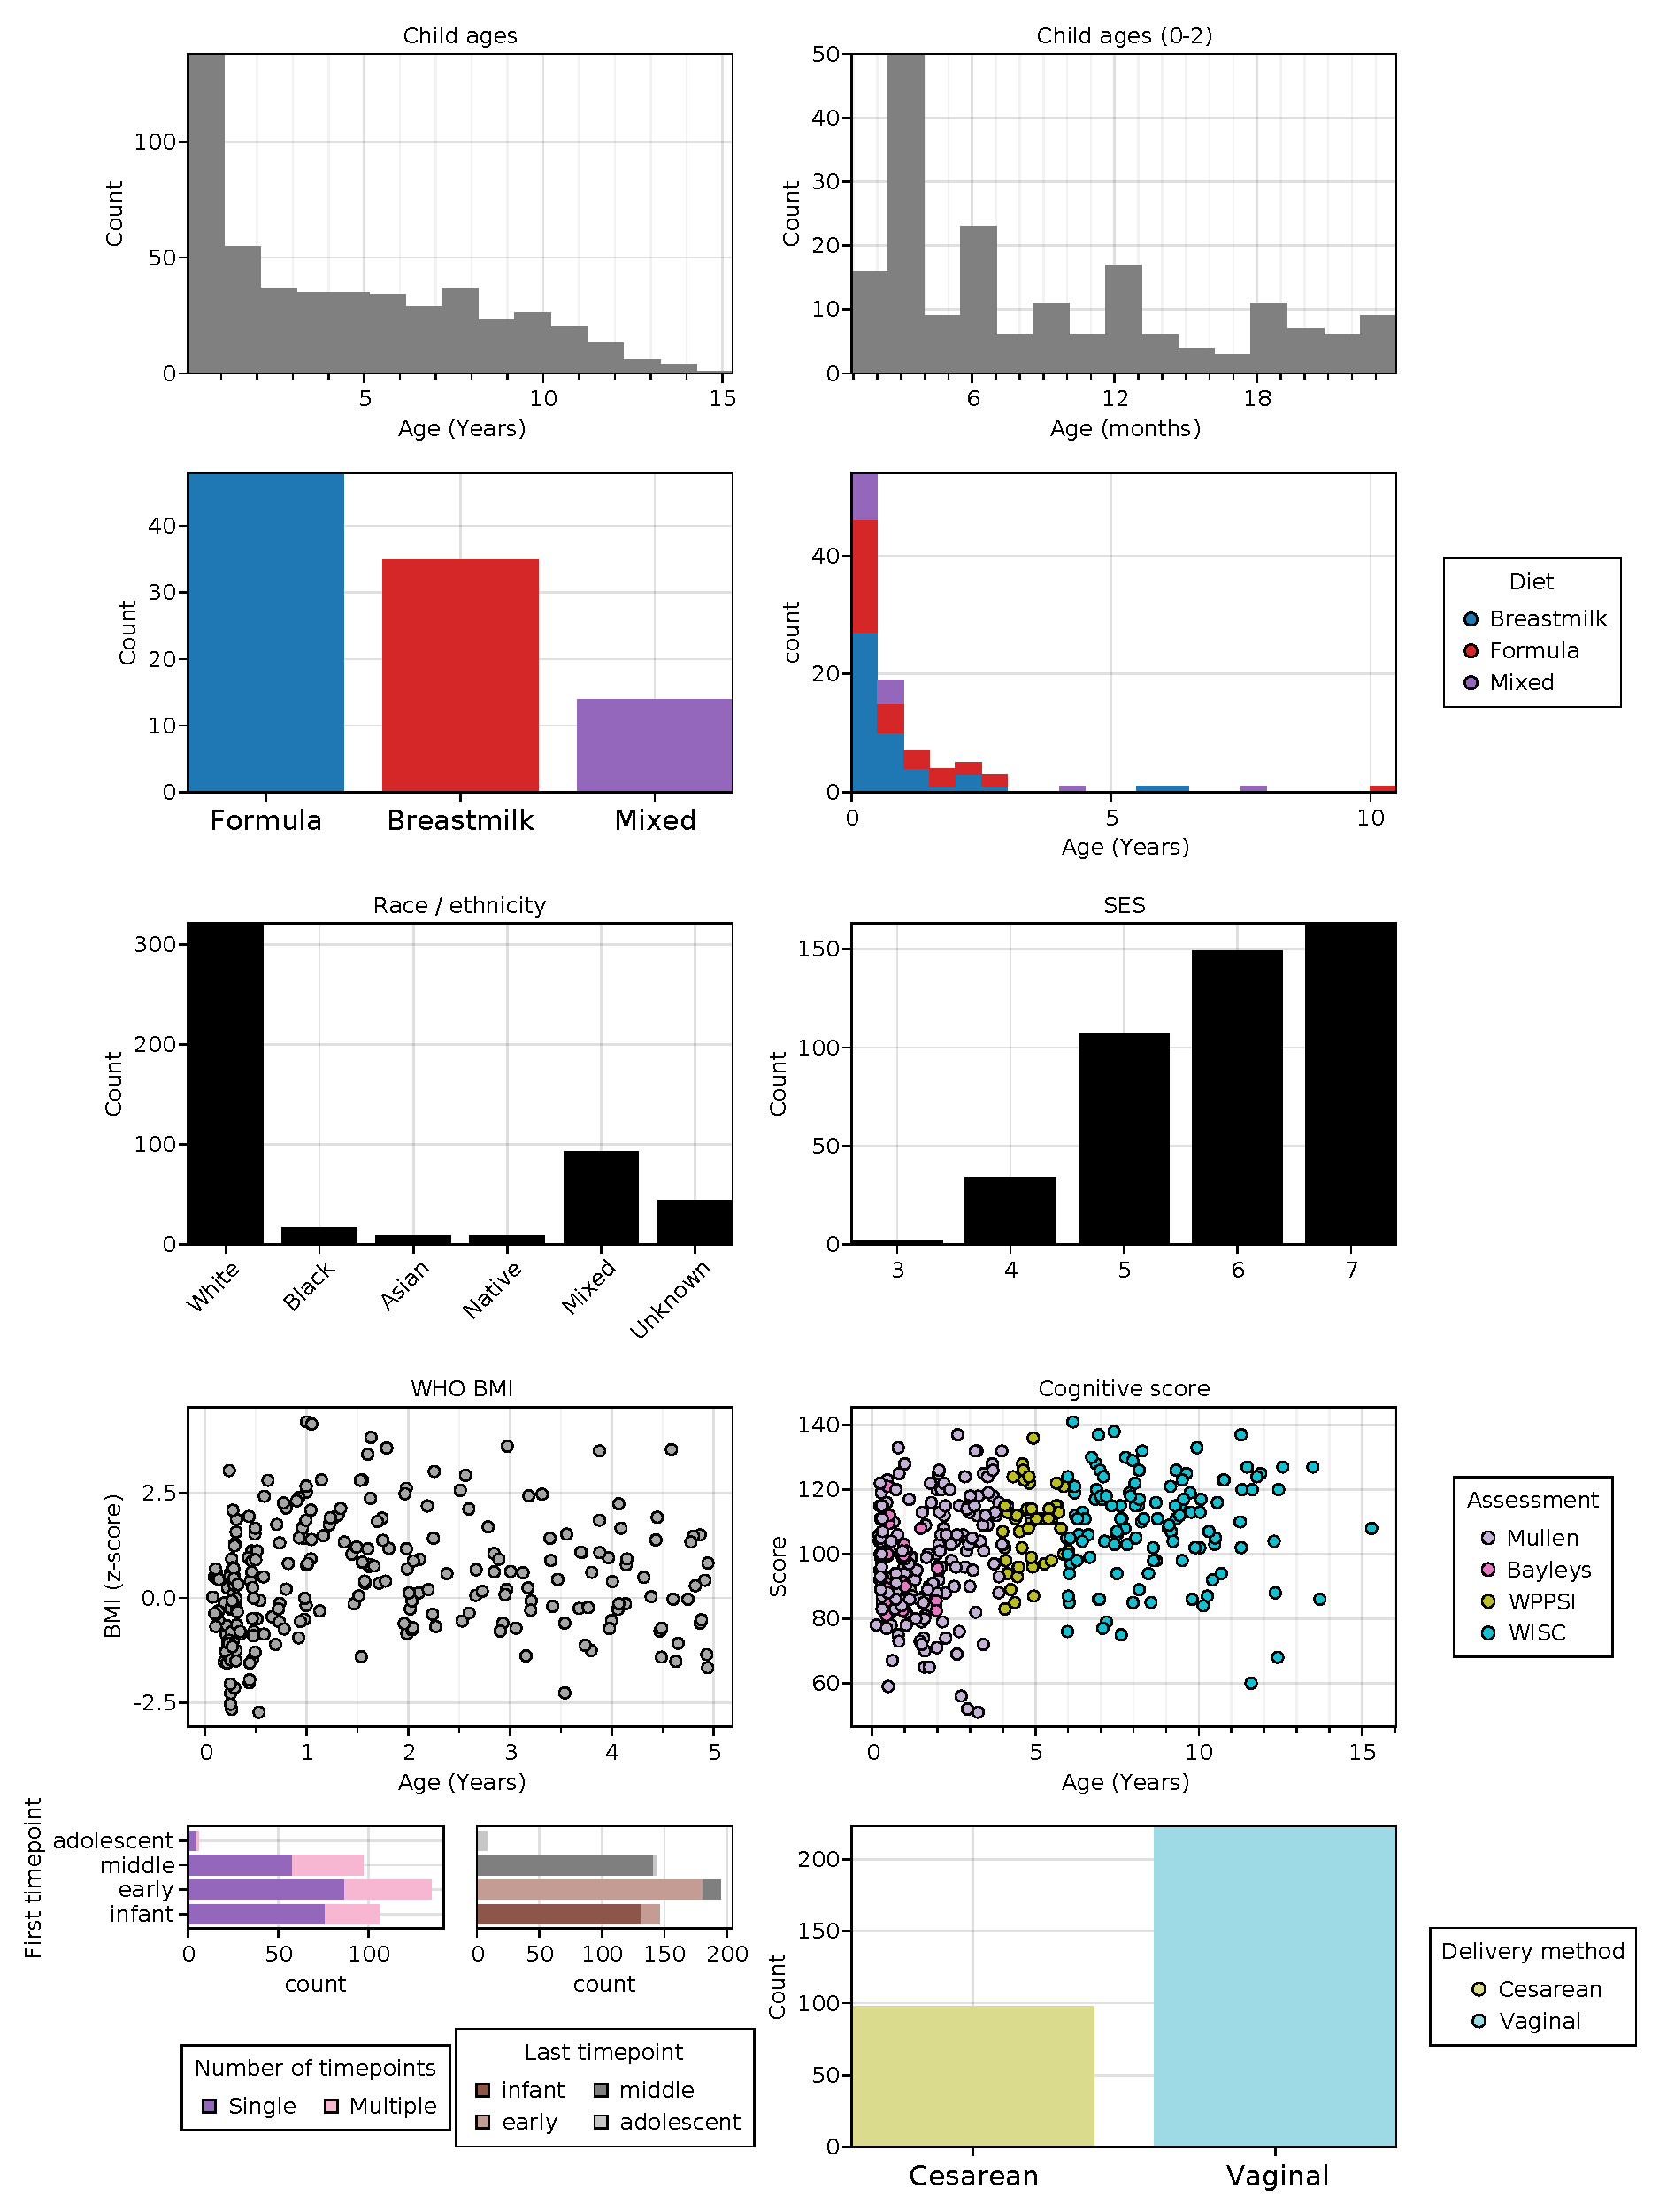
\includegraphics[width=\linewidth]{../figures/05_data_summaries}
\caption{
    Graphical representations of subject and sample-associated metadata.
    (a) Ages of children when samples were collected.
    (b) Age-normalized BMI z-score of children when samples were collected.
    (c) Age-normalized cognitive score of children when samples were collected.
    (d) Subjects with longitudinal timepoints by first collection.
}
\label{fig:data}
\end{figure}

\begin{figure}[ht]
\centering
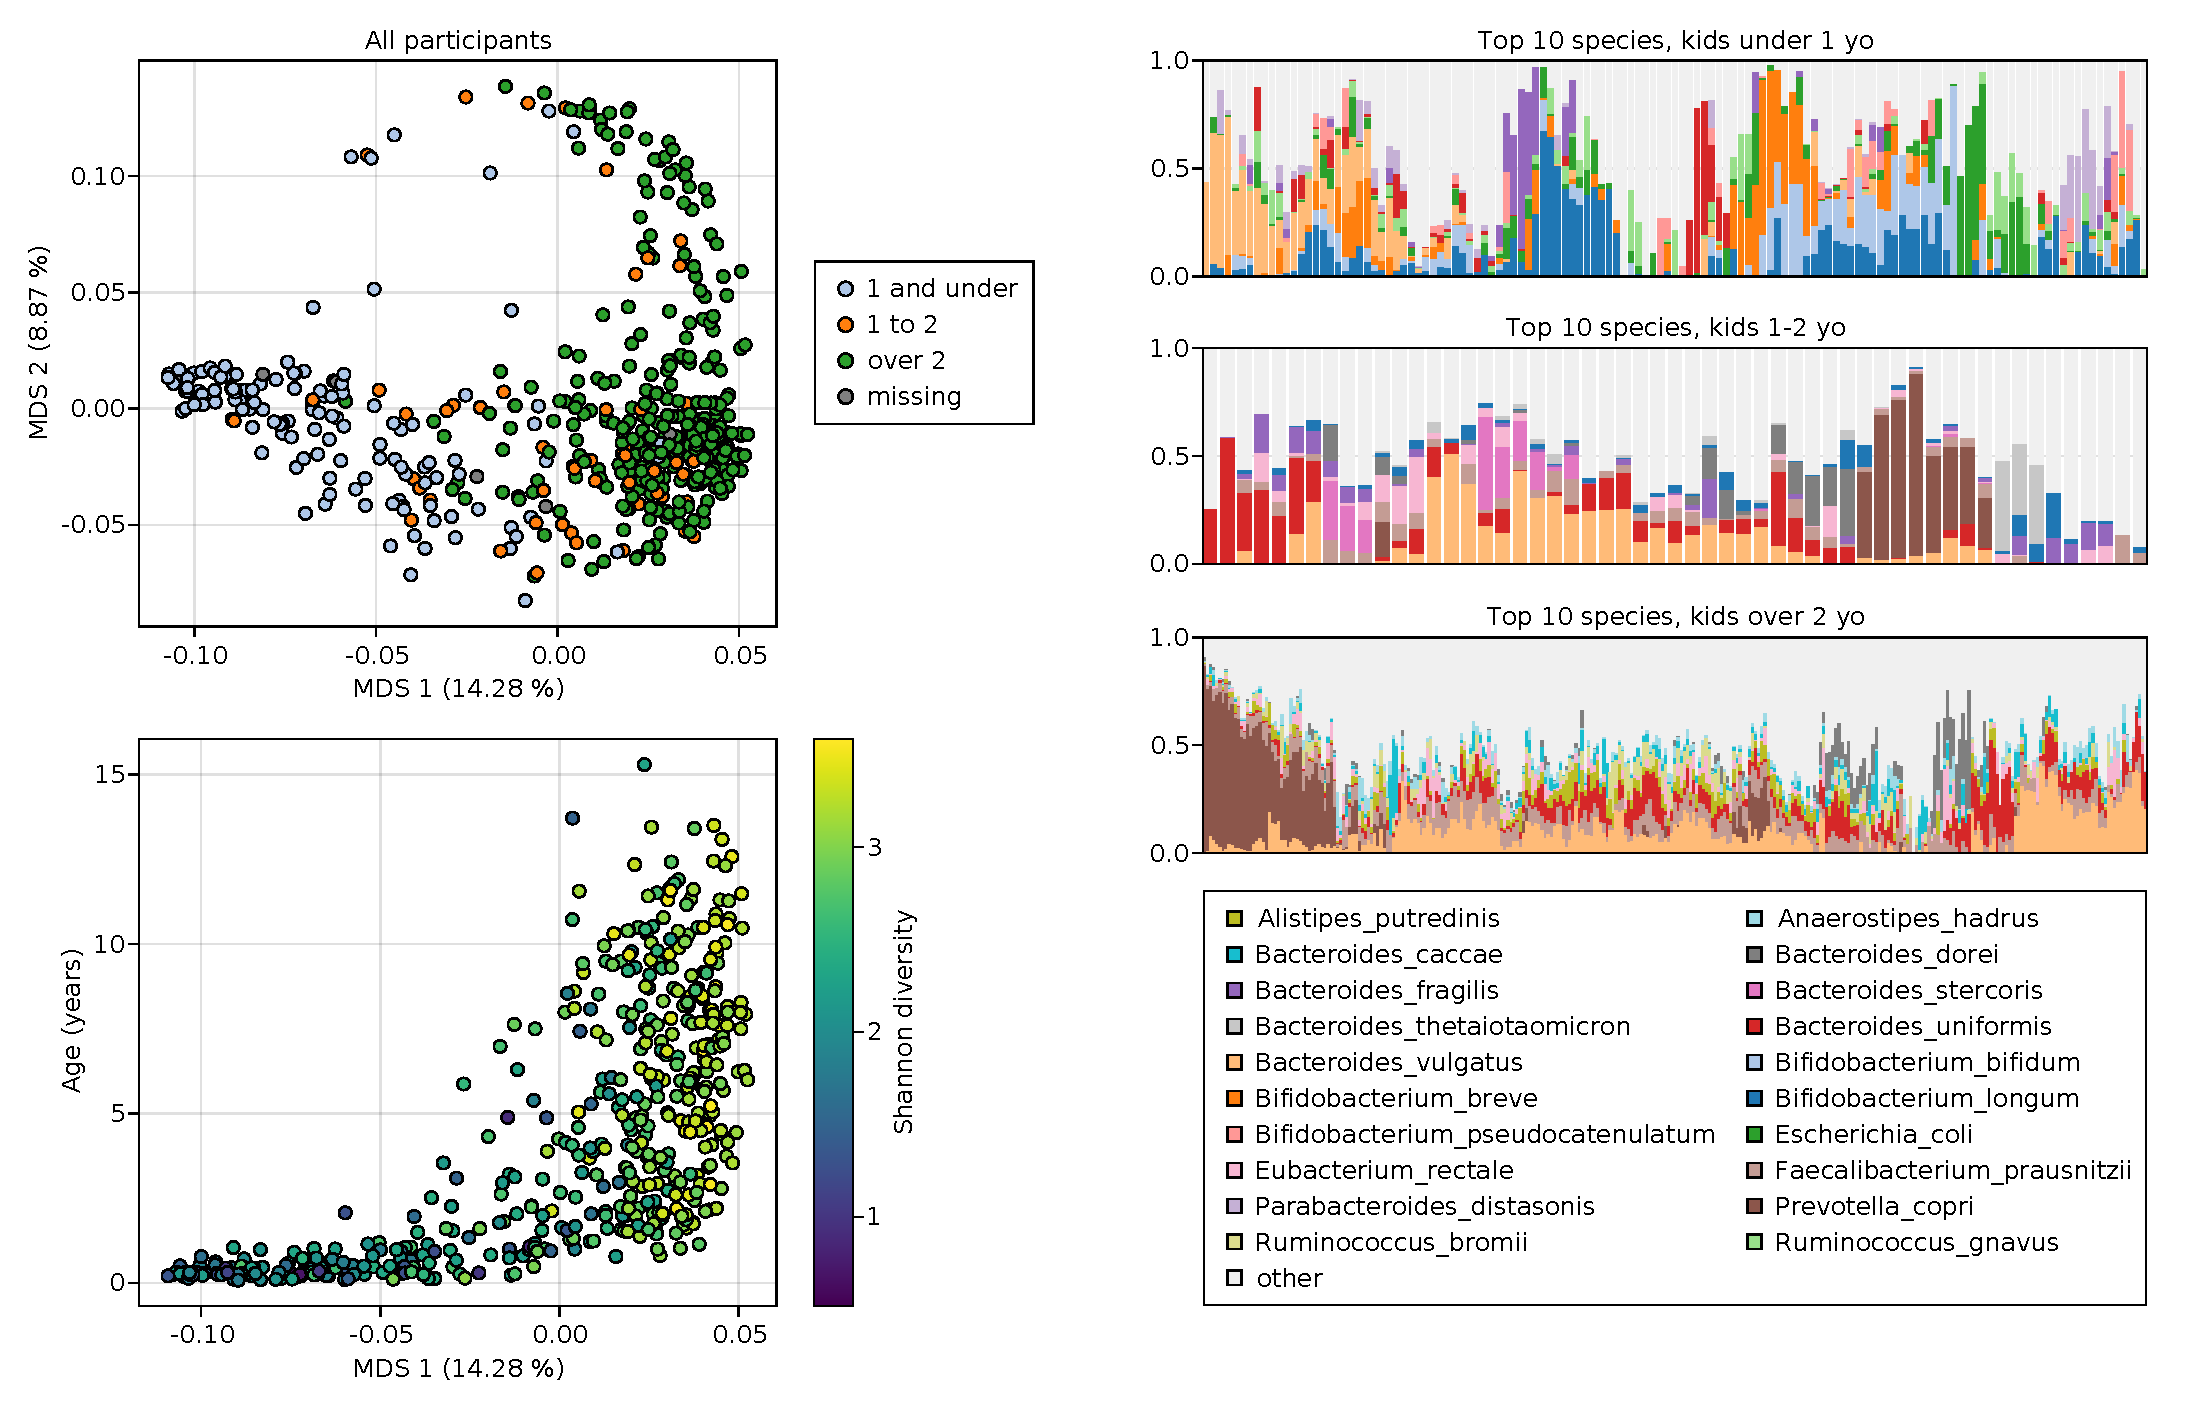
\includegraphics[width=\linewidth]{../figures/03_taxonomic_profiles}
\caption{
    Taxonomic profiles from metagenomic data.
    (a) Biplot of first two principal coordinate axes, colored by child age.
    (b) Principal coordinate 1 plotted against child age.
    (c) Top 10 taxa for each age group.
}
\label{fig:taxonomic}
\end{figure}

\begin{figure}[ht]
    \centering
    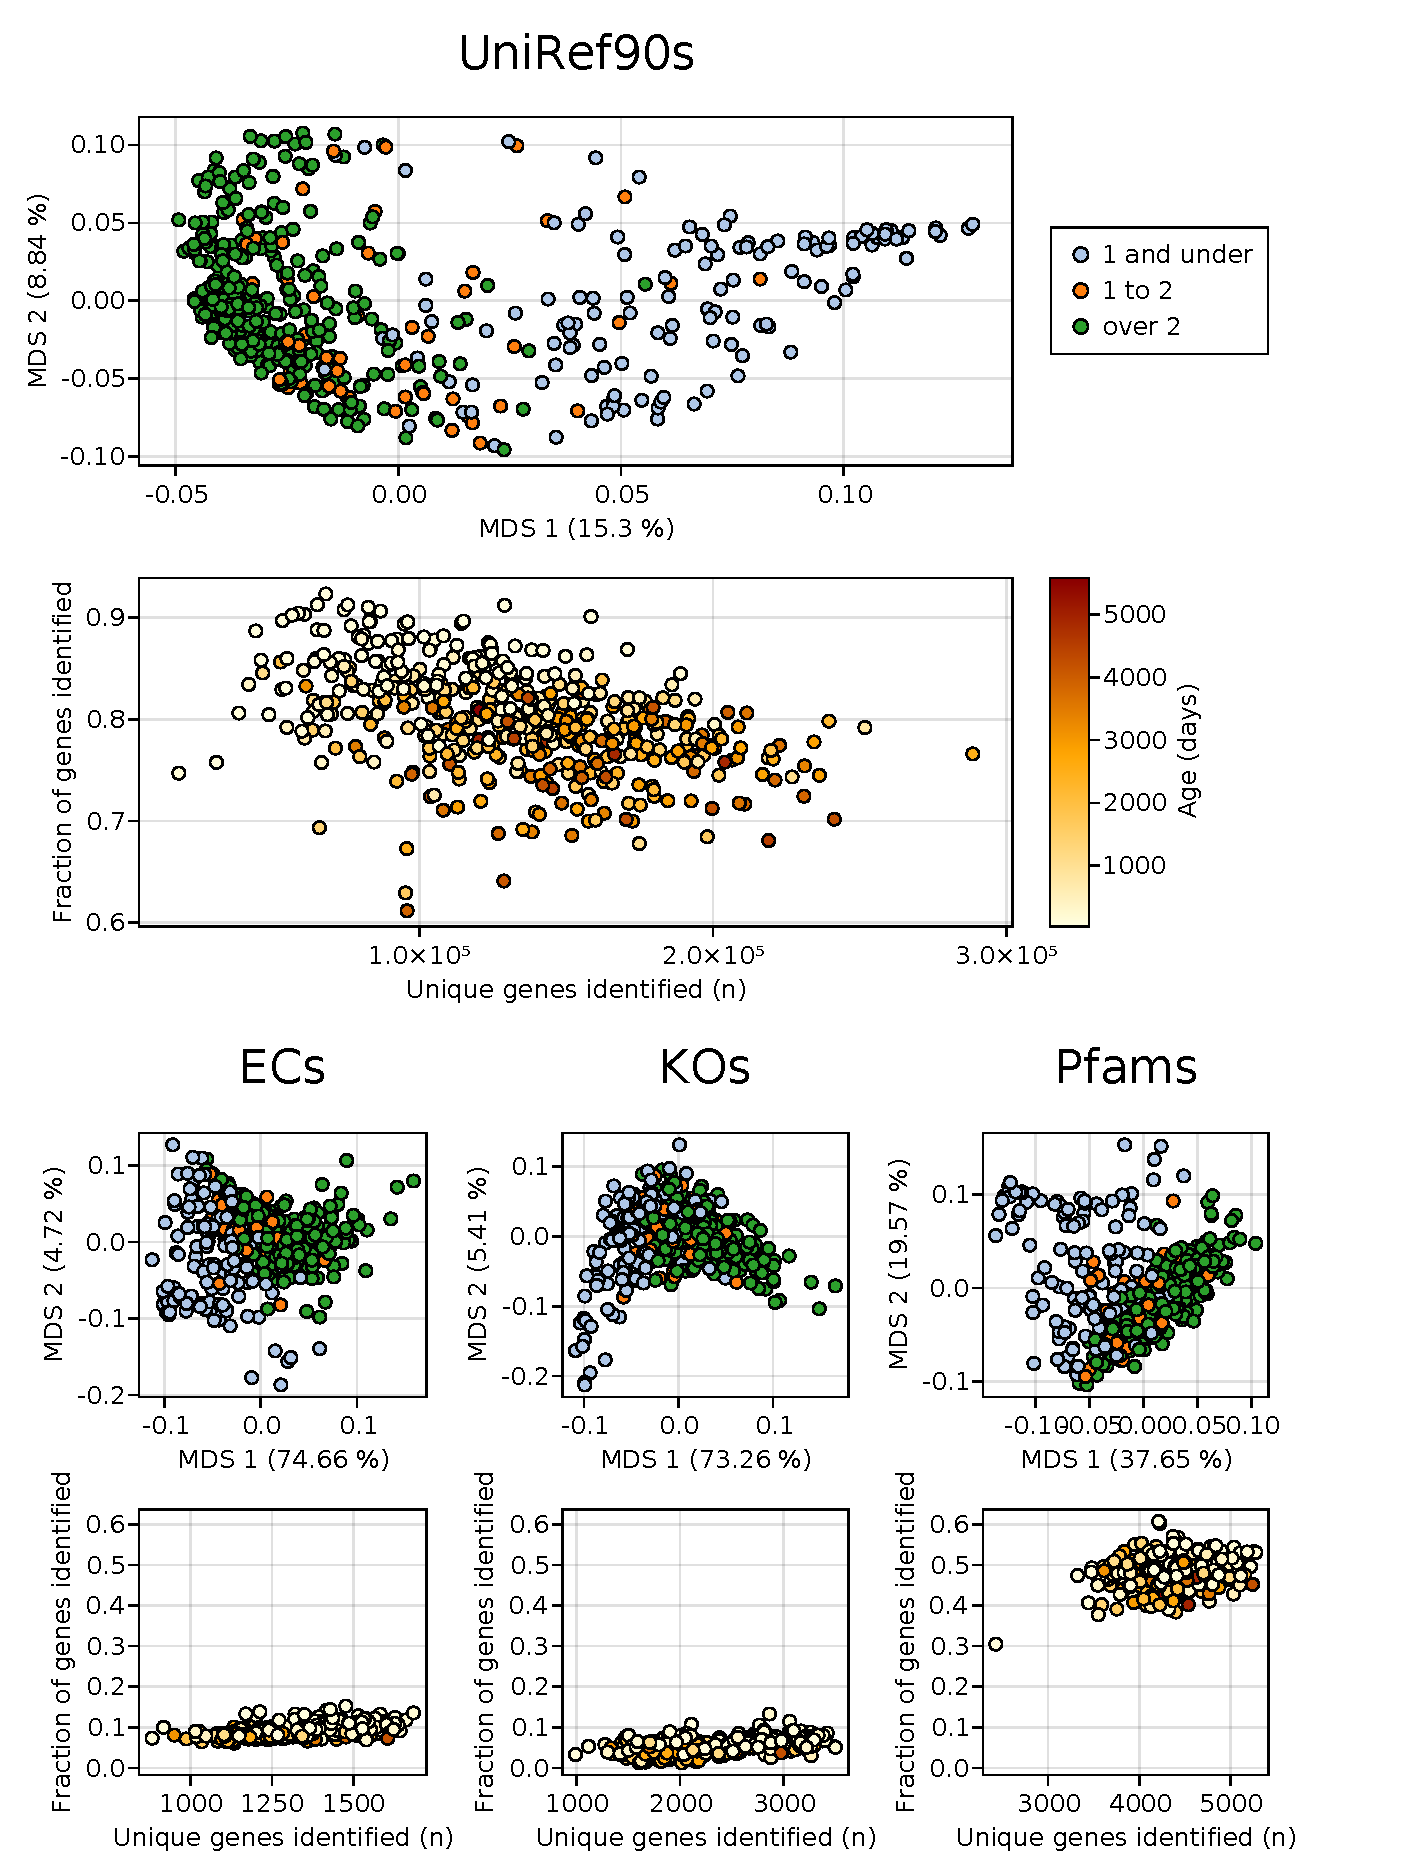
\includegraphics[width=\linewidth]{../figures/04_other_functions}
    \caption{
        Functional profiles from metagenomic data.
        (a-d) Biplots of top principal coordinates for each included functional profile modality.
        (e-i) Total number of unique gene functions and the percent of gene functions identified for each sample. 
    }
    \label{fig:functional}
    \end{figure}

\end{document}